\chapter{Методы кластеризации геораспределенных данных}
Геораспределенные данные~--- это данные о событиях, которые в качестве основных атрибутов и атрибутов временной метки имеют две географические координаты~\cite{RFFI}.

При автоматизированном сборе информации о предпочтениях жителей по перемещению возникает потребность работы с большими объемами геораспределенных данных. Поскольку в маршрутной сети количество остановочных пунктов ограничено, то возникает проблема создания выборки данных, оптимальным образом представляющая исходный объем геораспределенных данных. Для этого предлагается использовать методы кластеризации данных.

Сформулируем постановку задачи кластеризации геораспределенных данных.

Пусть \( X \)~--- входная выборка точек, полученная из картографических сервисов, \( k \)~--- ожидаемое число узлов (остановочных пунктов) во входной выборке. Требуется построить \( C \)~--- сеть из \( k \) остановочных пунктов, оптимальным образом охватывающие все точки из входной выборки \( X \).

Задача является задачей машинного обучения без учителя, но имеет некоторые специфические особенности. Во-первых, стандартные применяемые метрики для решения данной задачи не подходят: необходимо учитывать особенности местности, такие как реки, овраги и балки, автомобильные и железные дороги, здания и промышленные зоны. Существуют алгоритмы, способные на учет препятствий \cite{estivill, obstacles, cod}, но они не опираются на карту местности, а хранят информацию о препятствиях в некотором абстрактном виде. Во-вторых, поскольку на выходе необходимо получить сеть остановочных пунктов, то центры рассчитываемых кластеров должны находиться на участках дорожной сети, а не в произвольной географической точке.

В качестве базового алгоритма был выбран алгоритм k-средних ввиду его удобной расширяемости на поставленную задачу и вида входных данных, которые можно считать равномерно распределенными по рассматриваемой области, то есть в них нет четко выраженных кластерных структур.

Предлагается два способа расчета расстояний между географическими объектами. Первый способ заключается в использовании в качестве расстояний решение обратной геодезической задачи для рассматриваемых точек \cite{geodesic}. Второй способ заключается в использовании в качестве расстояний длину маршрута между двумя рассматриваемыми точками.

Для начала рассмотрим алгоритмы кластеризации, с помощью которых можно решать данную задачу, если внедрить в них описанные выше методы расчета расстояний и подобрать конкретные параметры управления под конкретную входную выборку.

\section{Проанализированные методы}
\subsection{Алгоритм Mean Shift}
Алгоритм Mean Shift (средний сдвиг)~--- это процедура определения положения максимумов функции плотности. Часто используется в работах по кластеризации, обработке изображений и визуальном трекинге \cite{ms, meanshift}. Пример работы можно посмотреть на рисунке~\ref{pic:km-ms}.

\begin{figure}[h!]
    \centering
    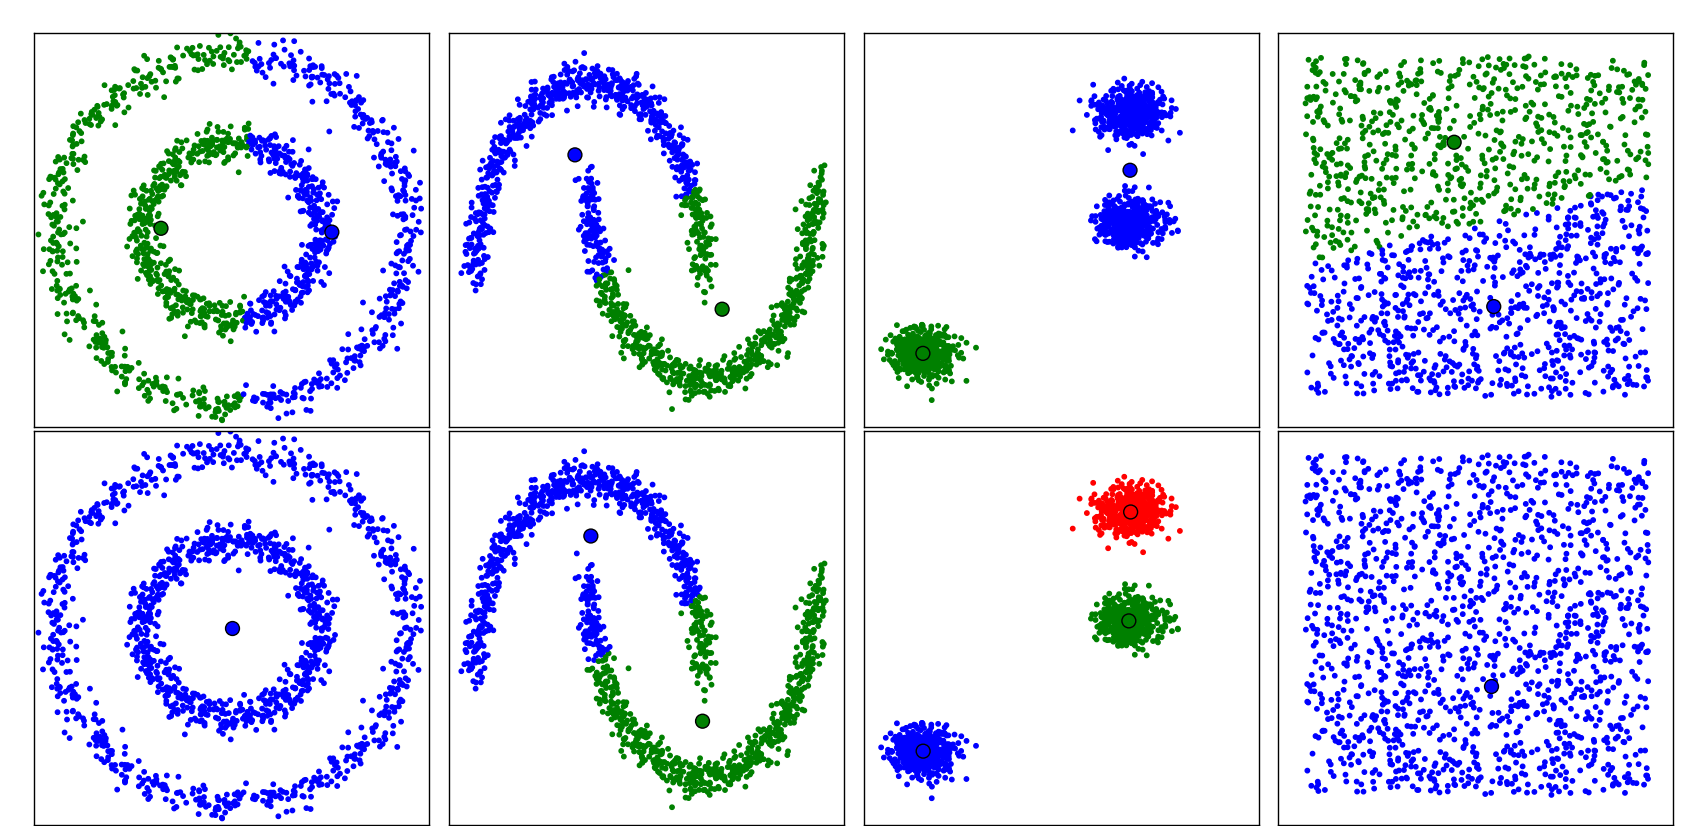
\includegraphics[width=.97\textwidth]{km_ms}\\[1ex]
    \parbox{.9\textwidth}{\caption{Результаты обработки одинаковых наборов данных алгоритмами k-means (верхний ряд) и mean shift (нижний ряд)} \label{pic:km-ms}}
\end{figure}

Пусть \( S\subset X \)~--- конечная выборка \( d \)-размерного пространства \( X \) из \( n \) элементов, \( K \)~--- функция ядра, \( w \)~--- весовая функция. <<Среднее выборки>> с ядром \( K \) в точке \( x\in X \) определяется функцией:
\begin{equation}
    m(x) = \frac{\ds\sum_{s\in S} K(s - x)w(s)s}{\ds\sum_{s\in S} K(s - x)w(s)}.
    \label{eq:wiki-shift}
\end{equation}
Пусть \( T\subset X \)~--- конечное множество центров кластеров. Изменение \( T \) итерационным присвоением \( T\gets m(T) = \Big\{ m(t), t\in T\Big\} \) называется алгоритмом среднего сдвига, или Mean Shift. Алгоритм останавливается, когда достигает фиксированного множества \( m(T) = T \) \cite{meanshift}.

Алгоритм основан на парзеновской оценке плотности:
\begin{equation}
    p_h(x) = \frac{1}{nh}\sum_{i=1}^n K\left(\frac{x - s}{h}\right),
    \label{eq:voron2.10}
\end{equation}
где \( h \)~--- неотрицательный параметр, называемый \emph{шириной окна}. Эмпирическая оценка плотности определяется как доля точек выборки \( S = (s)_{i=1}^n \), лежащих внутри отрезка \( [x - h, x + h] \).

Параметр \( h \) в формуле~\eqref{eq:voron2.10} называют шириной окна (пропускной способностью, англ. \emph{bandwidth}) алгоритма.

Ширина окна существенно влияет на качество определения сгустков плотности.

При \( h\to 0 \) сгустами плотности считаются все объекты выборки, функция~\eqref{eq:voron2.10} начинает претерпевать резкие скачки. При \( h\to\infty \) функция плотности чрезмерно сглаживается и вырождается в константу.

При сильно неравномерном распределении объектов выборки в пространстве \( X \) одно и то же значение ширины окна \( h \) может привести к недостаточному сглаживанию плотности в одних областях пространства \( X \) и наоборот, к сильному сглаживанию плотности в других областях. Для решения этой проблемы используют переменную ширину окна, определяемую в каждой точке \( x \) пространства \( X \). Тогда при расчетах используется матрица пропускной способности \( \matx{H} \)~--- симметричная положительная матрица размером \( d\times d\):
\begin{equation}
    p(x) = \frac{1}{n}\sum_{i=1}^n K_\matx{H}(x - s),
    \label{eq:msrobust1}
\end{equation}
где ядро \( K_\matx{H} \) представляется в виде:
\[
    K_\matx{H}(z) = \abs{\matx{H}}^{-1/2} K(\matx{H}^{-1/2}z).
\]

Зачастую при рассчетах матрицу \( \matx{H} \) считают диагональной:\linebreak \( \matx{H} = \matx{diag}\left(h_1^2, \ldots, h_d^2\right) \). При постоянной ширине окна матрицу можно представить в виде \( \matx{H} = h^2\matx{E} \), где \( \matx{E} = \matx{diag}(1, 1, \ldots) \)~--- единичная матрица.

Функция ядра \( K(z) \) является четной, нормированной и непрерывной, удовлетворяет следующим условиям:

\[
    \begin{array}{rl}
    \ds \int_X K(z)\,dz = 1; \qquad &
    \lim_{\norm{z}\to\infty} \norm{z}^d K(z) = 0; \\[1em]
    \ds \int_X zK(z)\,dz = 0; \qquad &
    \int_X zz^\T K(z)\,dz = c_K\matx{E},
    \end{array}
\]
где \( c_K \)~--- константа.

В алгоритме используется \emph{профильный} способ представления ядра, которым можно описать радиально-симметричные ядра, удовлетворяющие условию
\[
    K(z) = c_{k, d} k\left(\norm{z}^2\right).
\]

Функция \( k(z) \) называется профилем ядра, \( c_{k,d} > 0 \)~--- константа нормализации.

При таком способе представления ядра и постоянной ширине окна, \eqref{eq:msrobust1} можно переписать в виде:
\begin{equation}
    p_{h, K}(x) = \frac{c_{k, d}}{nh^d}\sum_{i=1}^n k\left(\norm{\frac{x - s}{h}}^2\right).
    \label{eq:msrobust11}
\end{equation}

Хотя функция ядра практически не влияет на качество кластеризации, она определяет степень гладкости функции~\eqref{eq:msrobust11}, и ее вид может повлиять на эффективность вычислений.

Зачастую для алгоритма Mean Shift используют определенные профили ядерных функций:
\begin{itemize}
    \itemsep-.5ex
    \item Плоское ядро:
        \( \ds k(z) = \left\{
            \begin{array}{ll}
                1 & \text{ если } z\le\lambda, \\
                0 & \text{ если } z > \lambda;
            \end{array} \right.
        \)
    \item нормальное (гауссовское) ядро:
        \( \ds k(z) = \exp\left(-\frac{\norm{z}^2}{2\sigma^2}\right), \)
        в котором параметр среднеквадратичного отклонения \( \sigma \) играет роль ширины окна \( h \);
    \item ядро Епачечникова:
        \( \ds k(z) = \left\{
            \begin{array}{ll}
                1 - z & \text{ если } 0\le z\le 1, \\
                0 & \text{ если } z > 1.
            \end{array} \right.
        \)
\end{itemize}

Формула~\eqref{eq:wiki-shift} представляет собой упрощенную запись отношения\linebreak \( m(x) = C\nabla p(x) / p(x) \). Выражение \( \nabla p \) является градиентом функции плотности:
\[
    \nabla p_{h, K}(x) = \frac{2c_{k, d}}{nh^{d+2}}\sum_{i=1}^n (x - s)k'\left(\norm{\frac{x - s}{h}}^2\right).
\]

Введя замену \( g(z) = -k'(z) \), получим следующее:
\[
    \nabla p_{h, K}(x) = p_{h, G}(x)\frac{2c_{k, d}}{h^2c_{g, d}}m_{k, G}(x),
\]
где \( G(z) = c_{g, d} g\left(\norm{z}^2\right) \), \( m_{k, G} \)~--- средний сдвиг. Отсюда получаем:
\[
    m_{k, G}(x) = \frac{h^2c_{g, d}}{2c_{k, d}}\frac{\nabla p_{h, K}(x)}{p_{h, G}}.
\]

Псевдокод алгоритма~\cite[с. 235-236]{algms} представлен на схеме~\ref{alg:meanshift}.
\begin{algorithm}[ht!]
    \caption{Алгоритм Mean Shift}
    \KwData{\( S \), \( h \).}
    \KwResult{\( C = \{C_j\}\)~--- список центров кластеров.}
    1. \For{каждой точки данных \( s \)}{
        Рассчитать градиент плотности
        \[
           \nabla p_{h, K}(x) = \frac{2c_{k, d}}{nh^{d+2}}\sum_{i=1}^n(s - x)g\left(\norm{\frac{x - s}{h}}^2\right)\text{\;}
        \]
    }
    2. \For{каждого центра \( C_j \)}{
        Сдвинуть позицию: \( C_j = C_j + m_{k, G}(x) \)\;
    }
    3. \lIf{центры кластеров \( C \) изменились}{перейти на шаг 1}\lElse{закончить выполнение}
    \label{alg:meanshift}
\end{algorithm}

\subsection{Алгоритм DBSCAN}
Алгоритм DBSCAN (англ. \emph{Density-Based Spatial Clustering of Application with Noise}, плотностный алгоритм кластеризации пространственных данных с присутствием шума) был предложен как решение проблемы разбиения данных на кластеры произвольной формы.

Поскольку большинство алгоритмов стараются минимизировать расстояние от элементов до центра кластера, то они создают кластеры, по форме приближенные к сферическим. Авторы DBSCAN экспериментально показали, что разработанный алгоритм способен распознать кластеры различной формы. Пример работы алгоритма можно посмотреть на рисунке~\ref{pic:km-dbscan}.

\begin{figure}[tb!]
    \centering
    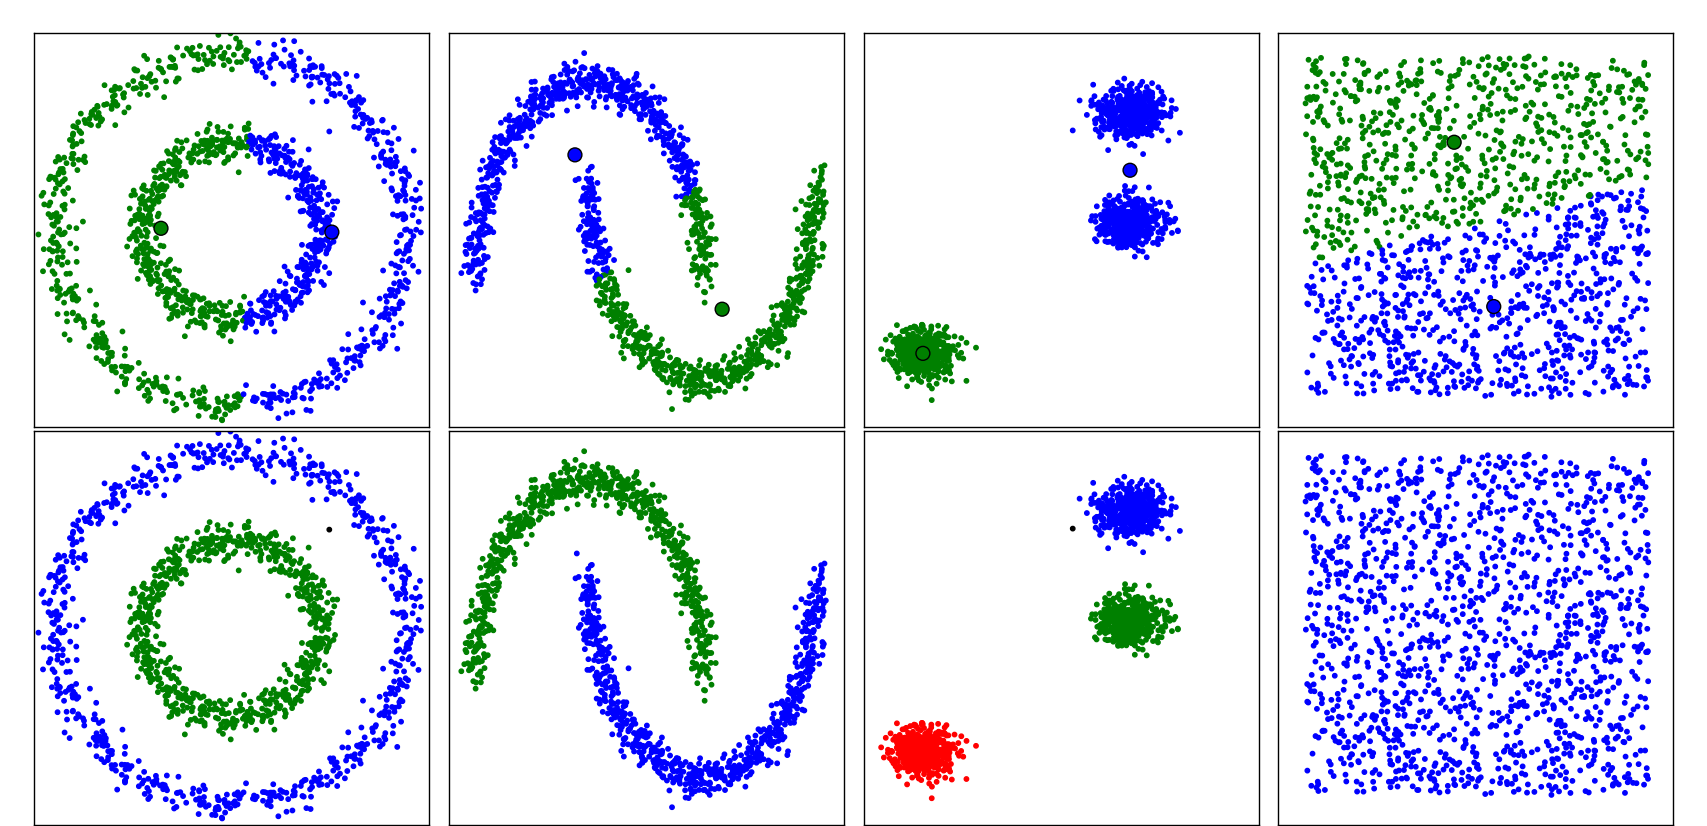
\includegraphics[width=.97\textwidth]{km_dbscan}\\[1ex]
    \parbox{.9\textwidth}{\caption{Результаты обработки одинаковых наборов данных алгоритмами k-means (верхний ряд) и DBSCAN (нижний ряд)} \label{pic:km-dbscan}}
\end{figure}

Алгоритм управляется двумя параметрами: \( \varepsilon \)~--- радиус области, на которой будет проводиться поиск соседних элементов, и \( \mu \)~--- минимальное количество соседних элементов в \( \varepsilon \)-окрестности, при котором элемент считается \emph{ядровым} элементом.

Основной концепт, положенный в основу работы алгоритма, заключается в том, что внутри каждого кластера плотность объектов обычно заметно выше, чем плотность объектов снаружи кластера, и плотность объектов в областях с шумом гораздо ниже плотности любого из кластеров~\cite{dbscan-pos}.

Реализация этого концепта была выражена следующими правилами~\cite{cod}:
\begin{itemize}
    \item объект может принадлежать кластеру только в том случае, если он лежит в \( \varepsilon \)-окрестности одного из ядровых элементов кластера;
    \item ядровый элемент \( o \), лежащий в \( \varepsilon \)-окрестности другого ядрового элемента \( p \), должен принадлежать тому же кластеру, что и \( p \);
    \item неядровый элемент \( q \), лежащий в \( \varepsilon \)-окрестности нескольких ядерных элементов \( p_1, \ldots, p_i \), должен принадлежать к тому же кластеру, к которому принадлежит хотя бы один из ядровых элементов;
    \item неядровый элемент \( r \), не лежащий в \( \varepsilon \)-окрестности ядровых элементов, считается шумовым элементом~--- элементом, не принадлежащему ни одному кластеру.
\end{itemize}

\begin{algorithm}[t!]
    \DontPrintSemicolon
    \KwData{\( X \), \( \varepsilon \), \( \mu \).}
    \KwResult{\( C = \{C_j\} \)~--- список кластеров.}
    1. Установить всем элементам \( X \) флаг = <<не посещен>>; \( j = 0 \); множество шума: \( N = \varnothing \);\;
    2. \ForEach{\( x\in X \) такого, что флаг == <<не посещен>>}{
        1. Флаг(\( x \)) = <<посещен>>\;
        2. \( n_x = \mathrm{Eps}(x) = \{q\in X | \rho(x, q)\le \varepsilon\}\);\;
        3. \lIf{\( \abs{n_x} < \mu \)}{N = N + \{x\}}\Else{
            номер следующего кластера \( j = j + 1\);\;
            \( \mathrm{ExpandCluster}(x, n_x, C_j, \varepsilon, \mu) \);\;
        }
    }
    \BlankLine
    \( \mathrm{ExpandCluster} \)\;
    \KwData{\( x \), \( n_x \), \( C_j \), \( \varepsilon \), \( \mu \).}
    \KwResult{кластер \( C_j \).}
    1. \( C_j = C_j + \{x\} \);\;
    2. \ForEach{\( q\in n_x \)}{
        1. \If{Флаг(q) == <<не посещен>>}{
            1. Флаг(q) == <<посещен>>;\;
            2. \( n_q = \mathrm{Eps}(q) \);\;
            3. \lIf{\( \abs{n_q}\ge \mu \)}{\( n_x = n_x + \{n_q\} \)}
        }
        2. \lIf{элемент \( q \) не принадлежит ни одному из кластеров}{\( C_j = C_j + \{q\} \)}
    }
    \caption{Алгоритм DBSCAN}
    \label{alg:dbscan}
\end{algorithm}

Чтобы обнаружить кластеры в данных, алгоритм DBSCAN просматривает \( \varepsilon \)-окрестности всех элементов входной выборки \( X \). Если в \( \varepsilon \)-окрестности элемента \( p \) находится больше, чем \( \mu \) элементов, то создается новый кластер с ядровым элементом \( p \). Все элементы в \( \varepsilon \)-окрестности ядрового элемента \( p \) добавляются в созданный кластер. Новые ядровые элементы в \( \varepsilon \)-окресности элемента \( p \) и элементы из их \( \varepsilon \)-окрестности также добавляются в созданный кластер; таким образом кластер разрастается. Как только в \( \varepsilon \)-окрестностях добавленных ядровых объектов больше нет элементов, то из выборки \( X \) берется следующий нерасмотренный ядровый элемент и создается новый кластер. Стоит отметить, что во время работы алгоритма ядровые элементы одного кластера могут быть обнаружены при разрастании другого, что приведет к слиянию кластеров. Алгоритм прекращает работу, когда нет новых точек, которые могут быть добавлены к какому-либо из кластеров.

Псевдокод алгоритма~\cite[с. 199]{dbscan-pos} представлен на схеме~\ref{alg:dbscan}. Используются следующие обозначения: \( \mathrm{Eps} \)~--- множество соседей элемента, находящихся от точки \( p \) на расстоянии не более \( \varepsilon \), \( N \)~--- множество элементов шума.

Существует улучшенная версия алгоритма DBSCAN, названная OPTICS (англ. \emph{Ordering Points To Identify Clustering Structure}, сортировка точек для определения кластерной структуры)~\cite{cod}. Он был создан для того, чтобы не запускать алгоритм DBSCAN множество раз с различными параметрами для получения оптимальной с точки зрения пользователя кластерной структуры. OPTICS также требует определения входных параметров \( \varepsilon \) и \( \mu \), но, в отличие от DBSCAN, при работе сортирует точки таким образом, чтобы легко визуализировать и рассчитать кластерную структуру для данного \( \varepsilon \) и некоторых других значений \( \varepsilon' < \varepsilon \).

\subsection{Алгоритм BIRCH}
Алгоритм BIRCH (англ. \emph{Balanced Iterative Reducing and Clustering using Hierarchies}, сбалансированное итерационное сокращение и кластеризация с использованием иерархий) создан для работы с большими наборами данных.

Пример работы алгоритма можно посмотреть на рисунке~\ref{pic:km-birch}.

\begin{figure}[h!]
    \centering
    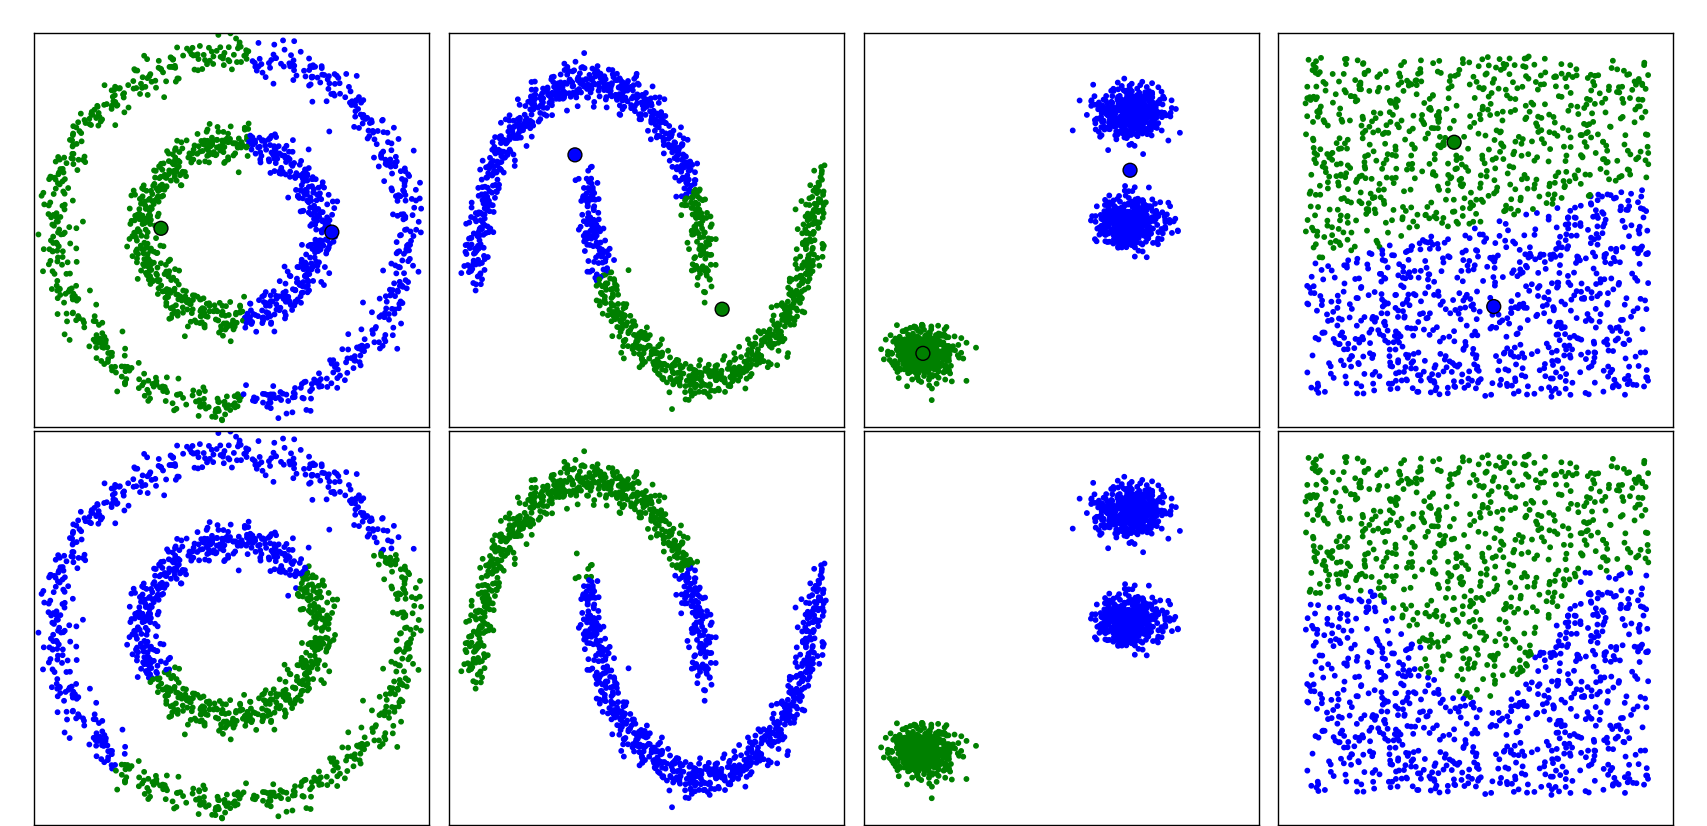
\includegraphics[width=.97\textwidth]{km_birch}\\[1ex]
    \parbox{.9\textwidth}{\caption{Результаты обработки одинаковых наборов данных алгоритмами k-means (верхний ряд) и BIRCH (нижний ряд)} \label{pic:km-birch}}
\end{figure}

Основная идея работы алгоритма BIRCH~--- сократить входную выборку до некоторого количества субкластеров, а затем провести кластеризацию над этими субкластерами~\cite{cod}. Из-за усечения множества исходных данных количество субкластеров гораздо меньше, чем число элементов входных данных, следовательно, это позволяет производить кластеризацию с меньшим количеством используемой памяти.

В алгоритме каждый небольшой субкластер представляется \emph{кластерным элементом} (англ. \emph{clustering feature}), который является триплетом, обобщающим информацию о группе объектов выборки, которую заменяет субкластер. Если в заданном \( d \)-размерном пространстве \( X \) субкластер заменяет \( N \) объектов выборки, то кластерный элемент определяется как
\[
    CF = \left(N, \vec{LS}, SS\right),
\]
где \( N \)~--- число заменяемых объектов выборки, \( \ds\vec{LS} = \sum_{i=1}^N \vec{X}_i \)~--- линейная сумма заменяемых объектов, \( \ds SS = \sum_{i=1}^N \vec{X}_i^2 \)~--- сумма квадратов заменяемых объектов.

Кластерные элементы хранятся в \emph{дереве кластерных элементов}, которое используется для иерархической кластеризации. Внутренние узлы дерева хранят суммы кластерных элементов их потомков и, следовательно, обобщенную информацию о потомках. Дерево кластерных элементов имеет два параметра: коэффициент ветвления \( B \) и пороговое значение \( T \). Коэффициент ветвления определяет максимальное количество потомков у внутренних узлов дерева. Пороговое значение определяет максимальный диаметр субкластеров, хранимых в листовых узлах дерева. Эти два параметра влияют на результирующий размер дерева.

Поскольку алгоритм рассчитан на работу с очень большими данными, то дерево строится сразу по мере считывания входной базы данных. Объекты вставляются в ближайший листовой элемент (субкластер). Если диаметр субкластера после добавления нового объекта становится больше порогового значения, то листовой узел разделяется и становится внутренним узлом. После добавления нового объекта информация о нем передается в корень дерева.

Если результирующее дерево выходит за границы доступной памяти, то изменяется пороговое значение \( T \) и дерево перестраивается, начиная с корня. Таким образом, процесс перестройки дерево происходит без повторного считывания всей исходной выборки.

После постройки результирующего дерева для кластеризации может использоваться любой алгоритм кластеризации, который не превысит границ доступной памяти.

Не смотря на достоинства алгоритма~--- линейную масштабируемость, хорошее качество кластеризации преобразованных данных,~--- узел в дереве кластерных элементов может содержать лишь ограниченное количество элементов из-за ограничения по размеру, что влечет за собой тот факт, что кластерное образование, наблюдаемое пользователем, может быть не отражено в дереве. Более того, если кластеры имеют несферическую форму, то алгоритм BIRCH не может корректно отразить этот факт, поскольку контроль за границами кластеров ведется через понятия радиусов и диаметров~\cite{cod, birch}.

Общее описание алгоритма приведено на схеме~\ref{alg:birch} \cite[с.~2]{neiskiy}.

\begin{algorithm}
    \DontPrintSemicolon
    Фаза 1. Загрузка данных в память.\;
    Построение начального дерева по данным (сканирование выборки).\;
    Фаза 2 (необязательная). Сжатие данных до приемлимых размеров.\;
    Перестройка и уменьшение дерева кластеных элементов с увеличением порогового значения \( T \).\;
    Фаза 3. Глобальная кластеризация.\;
    Применение выбранного алгоритма кластеризации на листовых элементах дерева.\;
    Фаза 4 (необязательная). Улучшение кластеров.\;
    Перераспределение данных между близкими кластерами, используя центры тяжести кластеров, полученные в фазе 3, как основы.\;
    \caption{Общая схема алгоритма BIRCH}
    \label{alg:birch}
\end{algorithm}

\vspace{-2ex}
\section{Алгоритм k-means} \label{sec:kmeans}
Так как алгоритм BIRCH чаще всего используют именно для работы с очень большими данными, о которых можно иметь репрезентативное представление в виде кластерных элементов~\cite{cod, birch, neiskiy}, то для кластеризации геораспределенных данных этот алгоритм не применялся.

Поскольку в работе рассматриваются данные, приближенные (но не являющиеся таковыми) к равномерно распределенным, то результатом работы алгоритма DBSCAN будет являться небольшое количество кластеров, включающих в себя большое количество точек.

Точно такое же поведение будет наблюдаться у алгоритма Mean Shift, но он более удобно настраивается, поскольку управляется одним параметром~--- шириной окна \( h \). При уменьшении этого параметра алгоритм проводит более детальную кластеризацию, однако результаты его работы слабо отличаются от результатов работы алгоритма k-means (рис.~\ref{pic:oldkm-ms}).
\begin{figure}[t!]
    \centering
    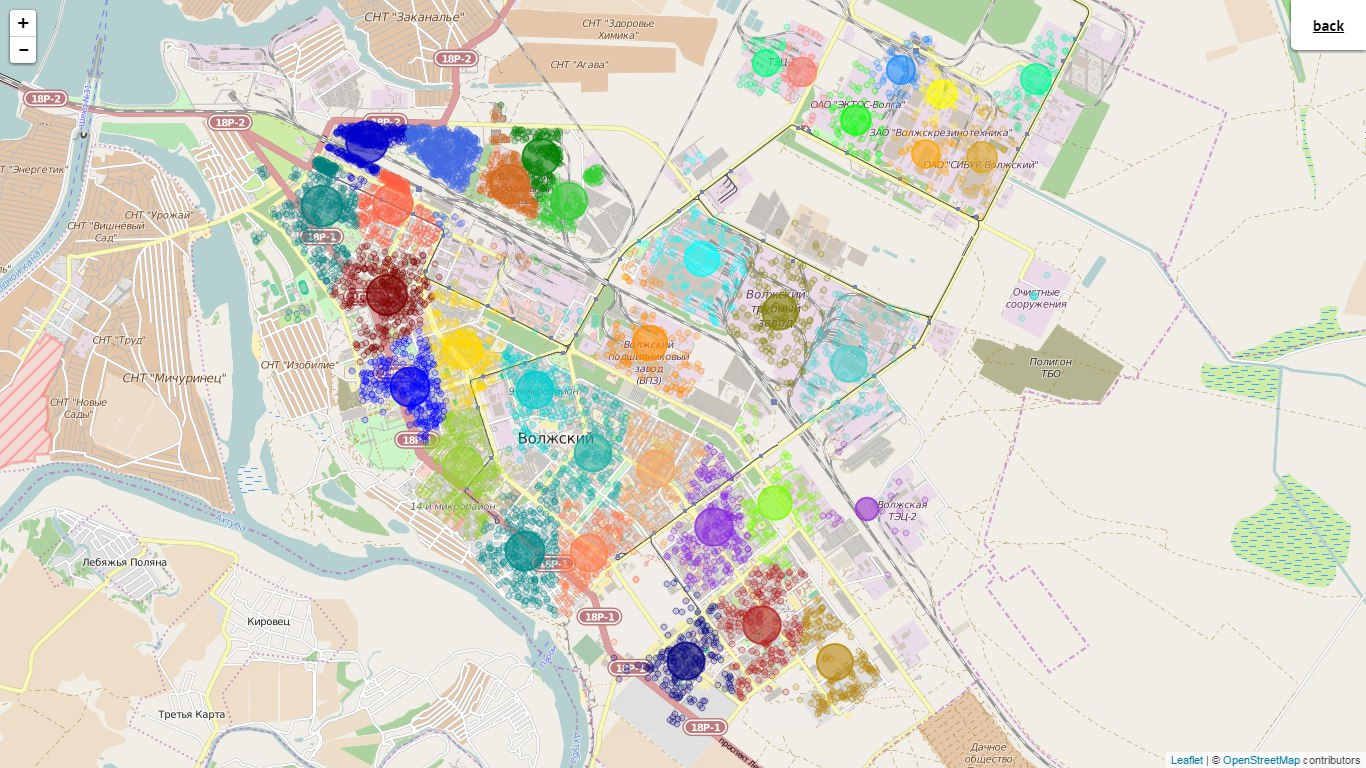
\includegraphics[width=.8\textwidth]{old_km}\\[.5ex]
    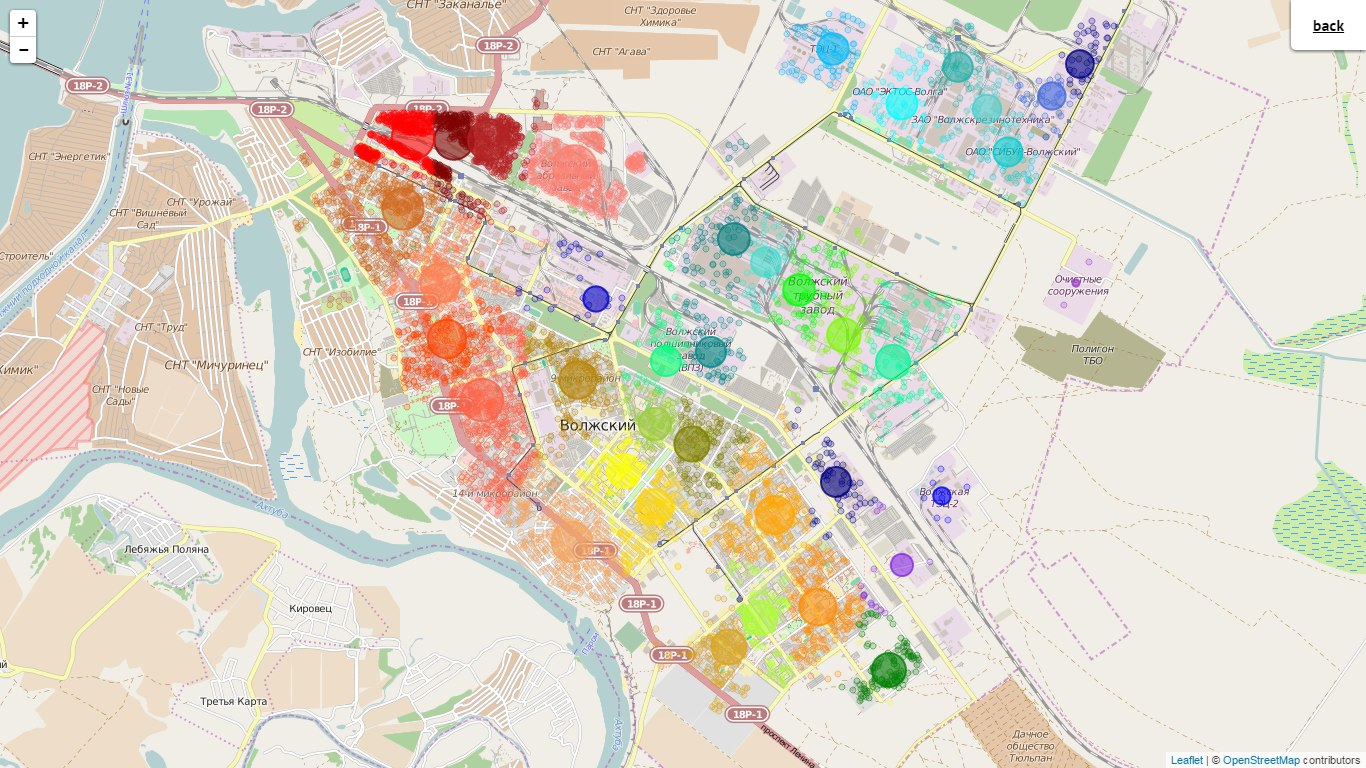
\includegraphics[width=.8\textwidth]{old_ms}\\[1ex]
    \parbox{.9\textwidth}{\caption{Результаты работы алгоритмов k-means (верхний) и Mean Shift (нижний) на сгенерированной входной выборке. Широкими кругами обозначены центры кластеров, радиус круга зависит от количества входящих в него точек}\label{pic:oldkm-ms}}
\end{figure}

\subsection{Общее описание}
Алгоритм k-means (k-средних) строит \( k \) кластеров, расположенных как возможно дальше друг от друга. Выбор числа \( k \) может базироваться на результатах теоретических соображений, предшествующих исследований, визуального наблюдения или иных источниках информации~\cite{neiskiy}.

Идеальным кластером алгоритм k-means считает сферу с центром кластера в центре сферы~\cite{dbscan-pos}.

При известном числе кластеров алгоритм k-средних начинает работу с некоторого начального расположения кластеров, к которым присваиваются объекты выборки.

Начальное расположение кластеров очень сильно влияет на работу алгоритма. Из-за неправильного выбора начальных значений алгоритм может попасть в некоторый локальный минимум целевой функции (рис.~\ref{pic:local_fail}).

\begin{figure}[ht!]
    \centering
    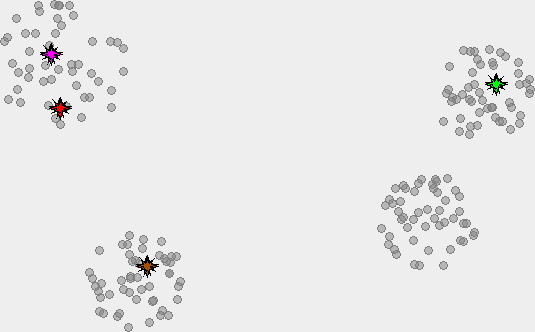
\includegraphics[width=.45\textwidth]{local_fail} \hspace{1em}
    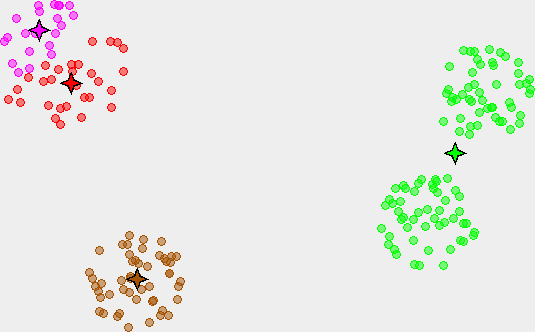
\includegraphics[width=.45\textwidth]{local_fail-2} \\[1ex]
    \parbox{.9\textwidth}{\caption{Пример сходимости алгоритма к локальному минимуму. Кружками обозначены объекты выборки, звездами~--- центры кластеров} \label{pic:local_fail}}
\end{figure}

Целевой функцией алгоритма является среднеквадратичное расстояние (при использовании евклидовой метрики) между объектами выборки и центрами их кластеров:
\[
    f(X, C) = \sum_{j=1}^k \sum_{i=1}^n \norm{x_i - \mu_j}^2,
\]
где \( \mu_j \)~--- центр кластера \( C_j \), вычисляющийся по формуле:
\begin{equation}
    \mu_j = \frac{1}{\abs{C_j}} \sum_{i=1}^n x_i.
    \label{eq:km-mu}
\end{equation}

Начальное расположение кластеров может задаваться как вручную, так и автоматически. В изначальном варианте алгоритма начальное расположение кластеров было случайным~\cite{macqueen}. На практике в качестве начальных центров кластеров зачастую либо выбирают первые \( k \) объектов выборки, либо выбирают \( k \) самых отдаленных друг от друга объектов выборки.

Алгоритм k-средних относительно масштабируем и эффективен при обработке не слишком больших баз данных поскольку его вычислительная сложность равна \( O(nki) \), где \( n \)~--- полное число объектов выборки, \( k \)~--- число кластеров, \( i \)~--- число итераций алгоритма; обычно \( k\ll n \) и \( i\ll n \)~\cite{cod}.

Недостатками алгоритма являются:
\begin{itemize}
    \item чувствительность к выбросам~--- точки, далеко находящиеся от всех кластеров, сильно искажают среднее;
    \item необходимость задавать количество кластеров~--- при работе с алгоритмом выбор числа кластеров является самым сложным вопросом. Если нет предположений о кластерной структуре данных, то рекомендуют постепенно наращивать число \( k \), сравнивая полученные результаты~\cite{neiskiy};
    \item необходимость сканировать всю выборку для определения положения каждого кластера~--- при работе с большими базами данных это сильно замедляет работу.
\end{itemize}

Достоинствами алгоритма являются его простота и быстрота использования, а также понятность и прозрачность алгоритма.

\subsection{Объяснение работы}
Работу алгоритма можно разбить на три этапа: начальный этап, этап присвоения и этап сдвига.

\begin{figure}[h!]
    \centering
    \raisebox{-1.5ex}{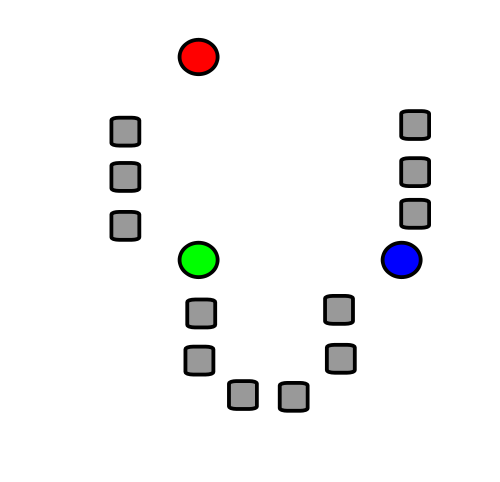
\includegraphics[width=.2\textwidth]{km_step1}} \hspace{1ex}
    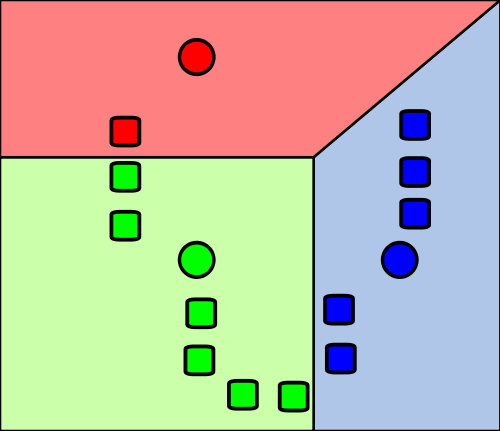
\includegraphics[width=.2\textwidth]{km_step2} \hspace{1ex}
    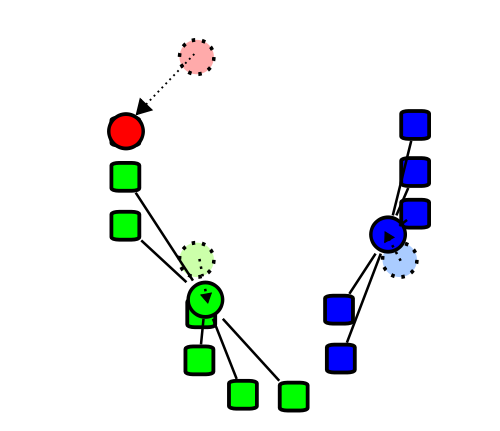
\includegraphics[width=.2\textwidth]{km_step3} \hspace{1ex}
    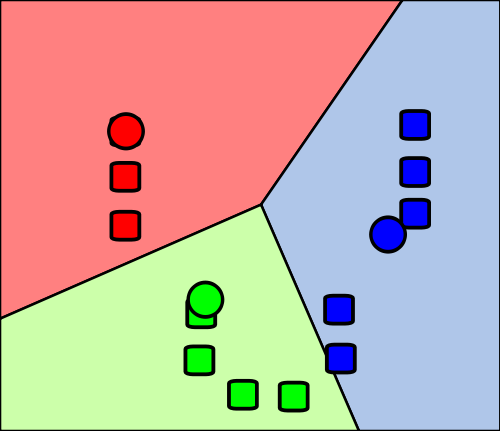
\includegraphics[width=.2\textwidth]{km_step4} \\
    \parbox{.2\textwidth}{\centering\small а)} \hspace{1ex}
    \parbox{.2\textwidth}{\centering\small б)} \hspace{1ex}
    \parbox{.2\textwidth}{\centering\small в)} \hspace{1ex}
    \parbox{.2\textwidth}{\centering\small г)} \\[1ex]
    \parbox{.9\textwidth}{\caption{Демонстрация работы алгоритма}\label{pic:km_steps}}
\end{figure}

На начальном этапе происходит выбор числа \( k \), расстановка начальных центров кластеров \( C_0 \) (рис.~\ref{pic:km_steps}а).

На этапе присвоения происходит расчет расстояния от каждого объекта выборки \( X \) до каждого объекта кластера \( C_j \). После чего считается, что объект принадлежит тому кластеру, до которого у него минимальное расстояние (рис.~\ref{pic:km_steps}б).

На этапе сдвига происходит расчет нового положения центров кластеров по формуле~\eqref{eq:km-mu} (рис.~\ref{pic:km_steps}в).

Этапы присвоения и сдвига повторяются, пока кластерные центры не стабилизируются, то есть все объекты, принадлежащие кластеру на прошлой итерации, принадлежат и на этой, либо пока не достигнется заданное максимальное число итераций \( I \). На выходе алгоритм выдает множество центров кластеров \( C \) и метки принадлежности объектов выборки кластерам \( L \) (рис.~\ref{pic:km_steps}г).

Псевдокод алгоритма представлен на схеме~\ref{alg:kmeans}.
\begin{algorithm}
    \KwData{\( X \), \( k \), \( C_0 \), \( I \).}
    \KwResult{\( C \), \( L \).}
    1. \( C = C_0 \), \( L_0 = \varnothing \), \( i = 0\)\;
    2. \While{\( L != L_0\) и \( i < I \)}{
        1. \( L_0 = L \), \( A = \varnothing \), \( \mu = \varnothing \)\;
        2. \ForEach{\( x \in X \)}{
            1. \( r = \varnothing \)\;
            2. \ForEach{\( c \in C \)}{
                1. Рассчитать \( r_{xc} = \rho(x, c) \)\;
                2. \( r = r + \{ r_{xc} \} \)\;
            }
            3. \( L[x] = C[\max(r)] \)\;
            4. \( A[C[\max(r)]] = A[C[\max(r)]] + \{x\}\)\;
        }
        3. \ForEach{\( c \in C \)}{
            1. \( \mu[c] = \sum(A[c])\,/ \abs{A[c]} \)\;
            2. \( c = \mu[c] \)\;
        }
        4. \( i = i + 1 \)\;
    }
    \caption{Алгоритм k-means}
    \label{alg:kmeans}
\end{algorithm}

\section{Расчет расстояний между точками} \label{sec:distance}

Особая метрика при работе алгоритма необходима по той причине, что два близких по стандартным метрикам геораспределенных объекта в реальности могут преграждаться препятствиями. Примеры таких объектов приведены на рисунке~\ref{pic:2points}. На рисунке~\ref{pic:2points-1} приведено реальное расстояние между объектами, которое должно учитываться при транспортных расчетах.

Для расчета расстояния между точками в работе используются две метрики, названные <<Surface>> и <<Route>>.

Метрика \emph{Surface} рассчитывает расстояние путем решения обратной геодезической задачи~\cite[с. 48-50]{geodesic}. Метрика \emph{Route} рассчитывает расстояние между объектами по графу городских дорог.

\begin{figure}[t!]
    \centering
    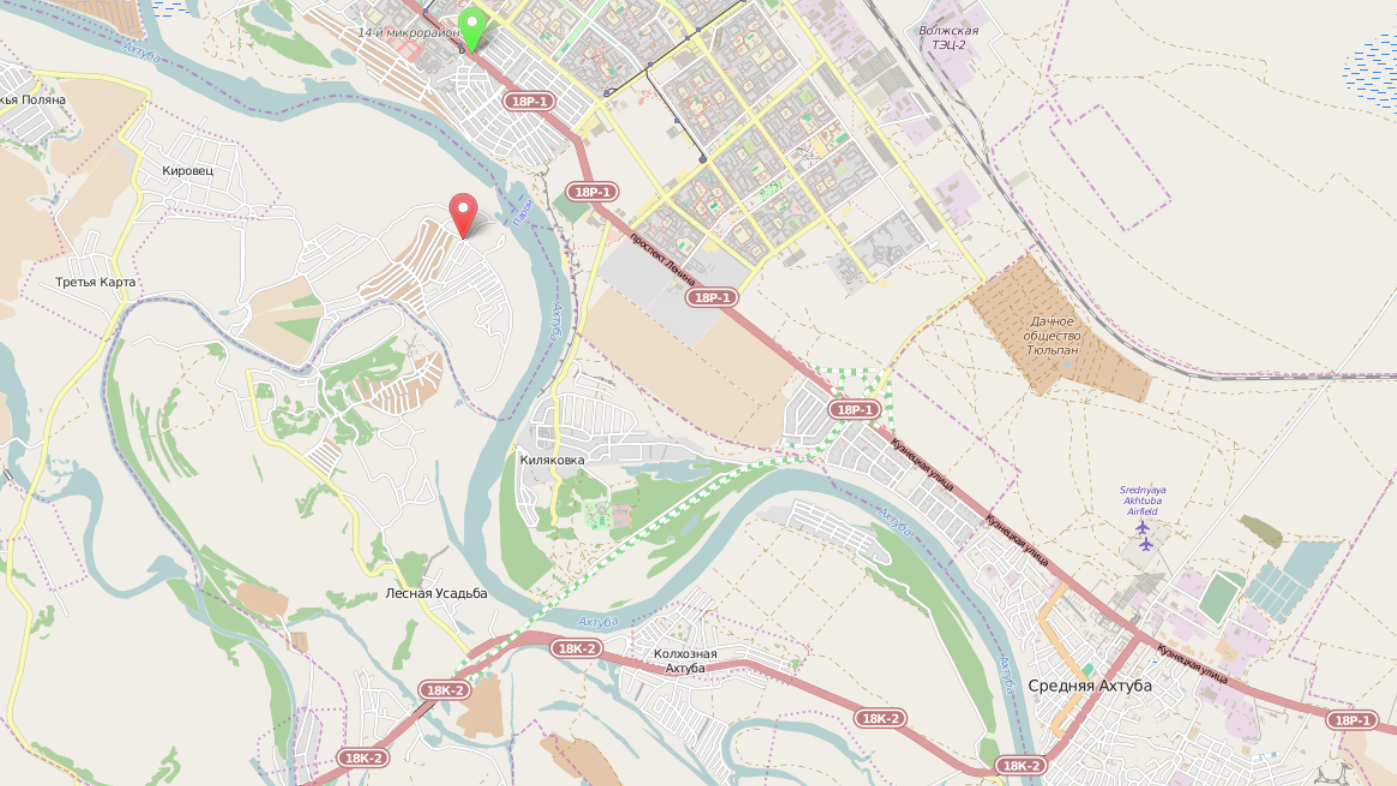
\includegraphics[width=.47\textwidth]{2points_1} \hspace{1ex}
    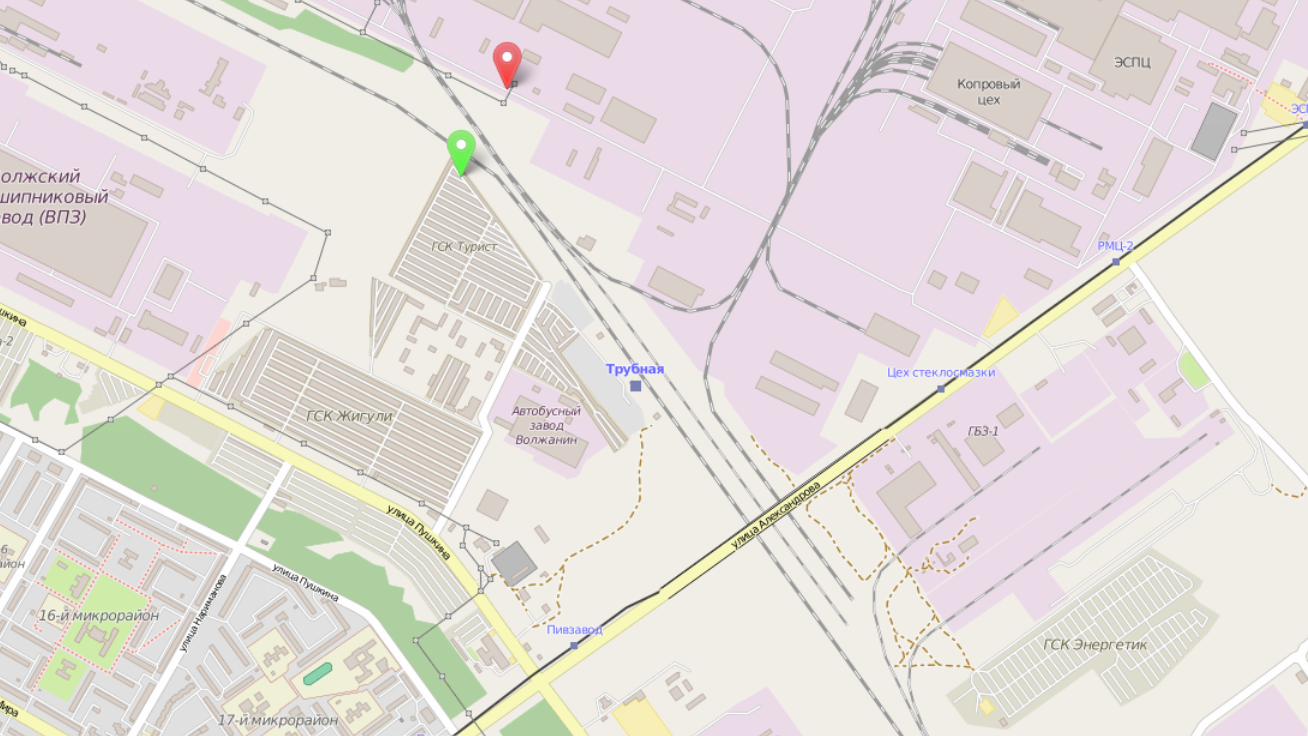
\includegraphics[width=.47\textwidth]{2points_3} \\[.5ex]
    \parbox{.9\textwidth}{\caption{Близкие по евклидовой метрике пары объектов}\label{pic:2points}}
    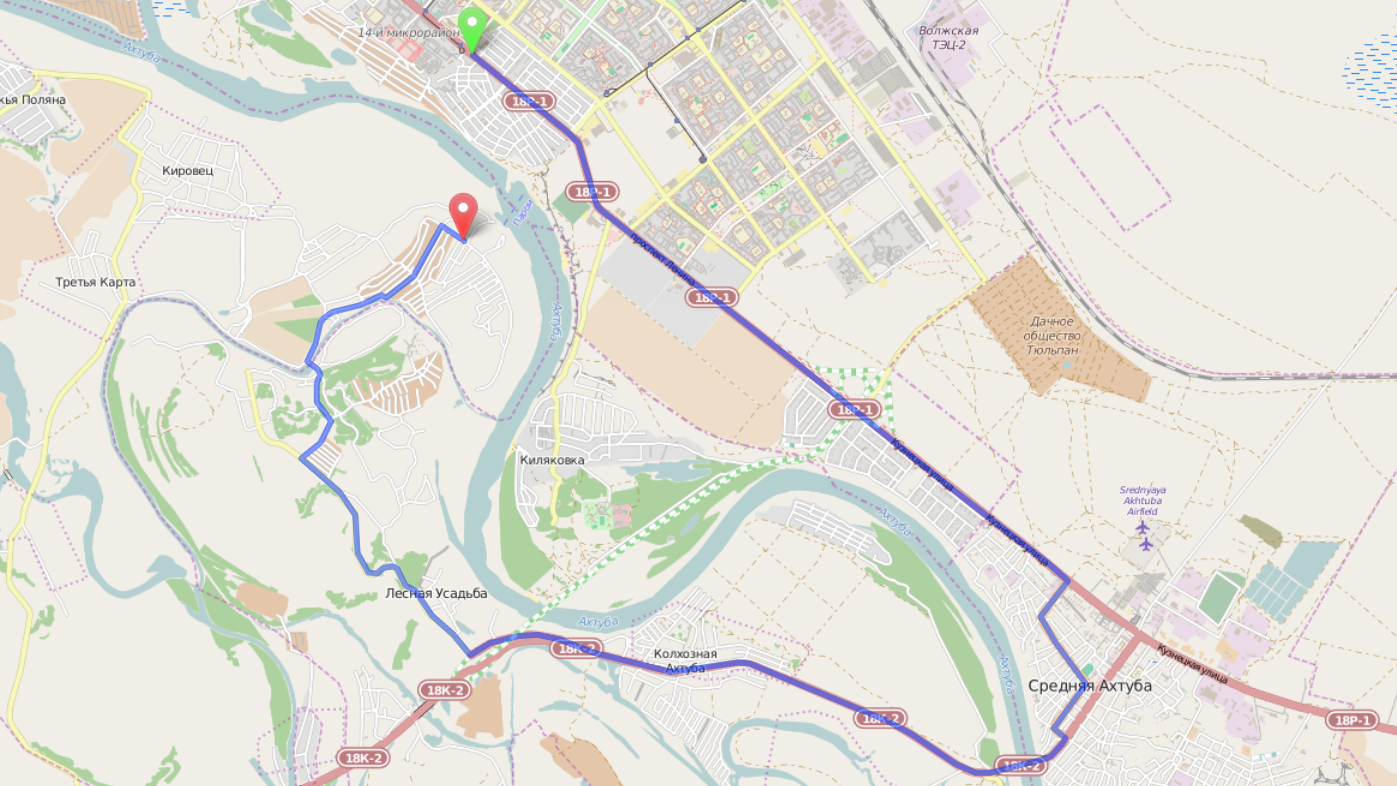
\includegraphics[width=.47\textwidth]{2points_2} \hspace{1ex}
    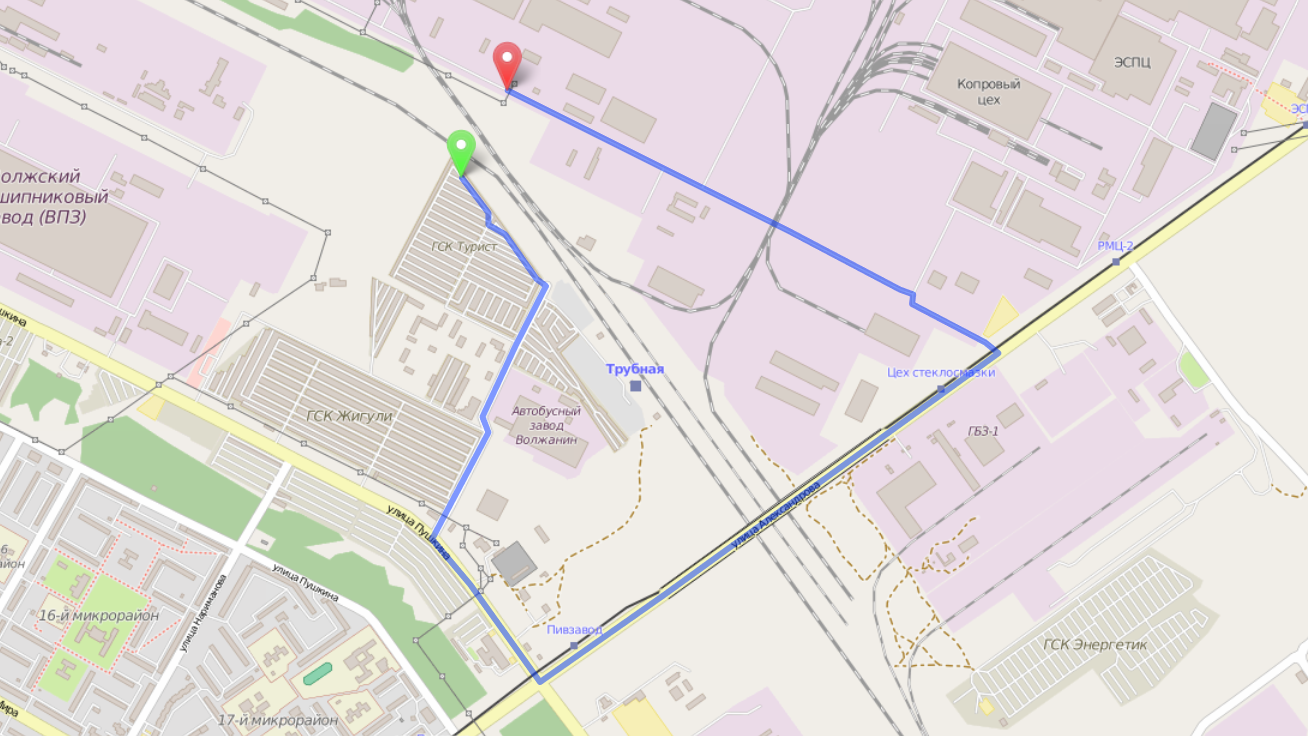
\includegraphics[width=.47\textwidth]{2points_4} \\[.5ex]
    \parbox{.9\textwidth}{\caption{Расстояние между объектами, которое должно учитываться при расчете}\label{pic:2points-1}}
\end{figure}

Для решения обратной геодезической задачи в метрике \emph{Surface} используется библиотека \emph{GeographicLib}~\cite{geographiclib}. Метрика использует сервис построения маршрутов \emph{Open Source Routing Machine} (OSRM)~\cite{OSRM} для расчета расстояния между точками по городским дорогам.

\begin{figure}[b!]
    \centering
    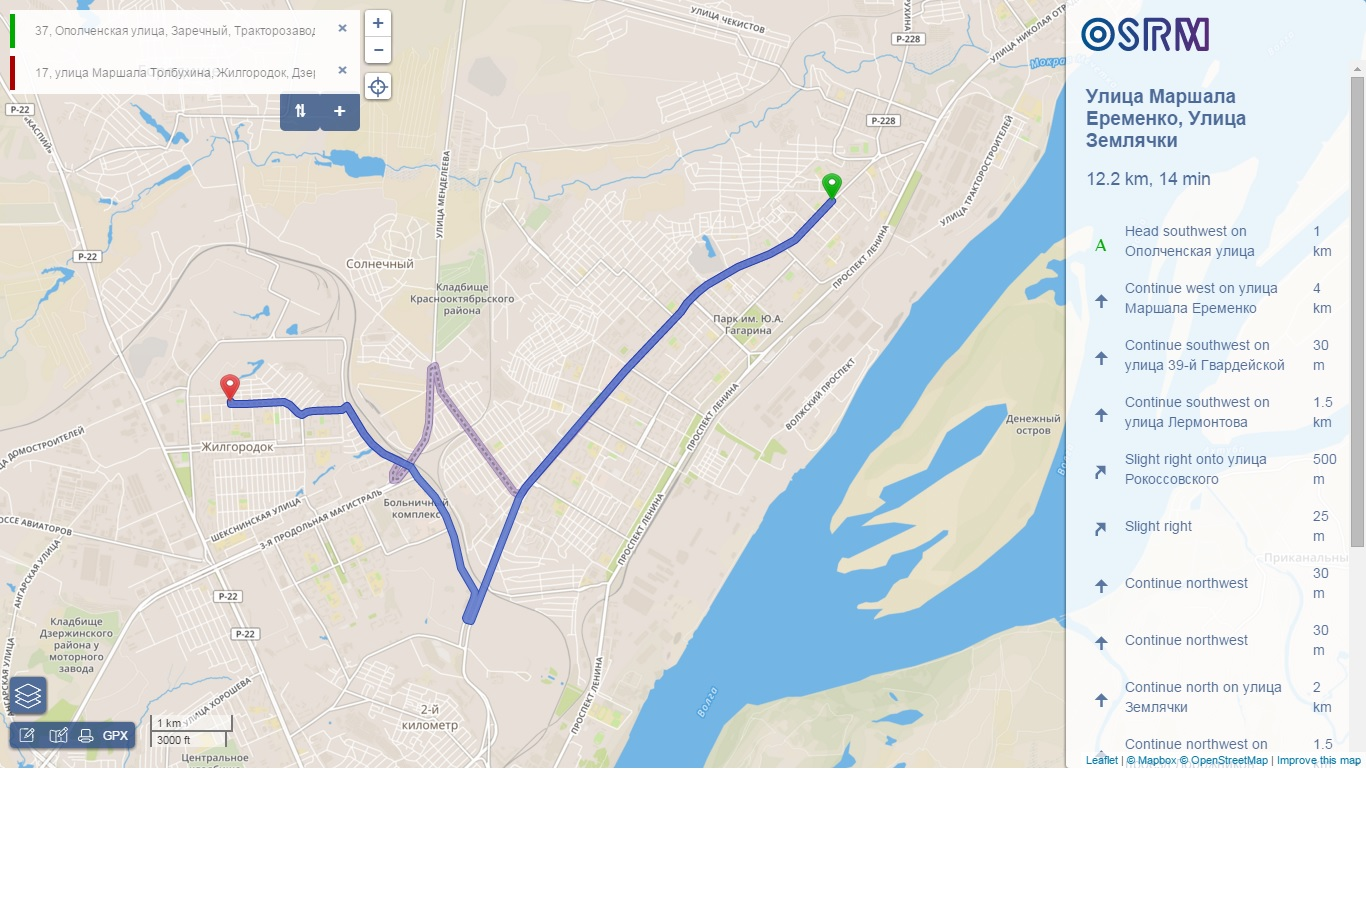
\includegraphics[width=.7\textwidth]{osrm}\\[1ex]
    \parbox{.9\textwidth}{\caption{Пример работы сервиса Open Source Routing Machine}\label{pic:osrm}}
    \vspace*{-1ex}
\end{figure}

Сервис OSRM предоставляет открытый код своего движка маршрутизации. Для работе с собранным движком на пользовательском компьюре используется HTTP-запросы определенной структуры. Результат обработки запроса выводится в json-формате, содержащем всю информацию по запросу.

Для работы движок маршрутизации должен распаковать карту сервиса \emph{Open Street Map}~\cite{OSM} для выделения на ней графа дорог. Главным параметром при работе с движком маршрутизации является используемый профиль (англ. \emph{profile}). При сборке OSRM из исходных кодов предоставляется несколько профилей, среди который профили автомобиля, велосипеда и пешехода. Используемый профиль влияет на способ построения маршрута и выбор городских дород для его прокладки. Пример работы сервиса Open Source Routing Machine представлен на рисунке~\ref{pic:osrm}.

\section{Заключение}
В данной главе были рассмотрены алгоритмы кластеризации, которые можно использовать при внедрении соответствующих метрик и точной настройке параметров для кластеризации геораспределенных данных: алгоритмы Mean Shift, DBSCAN и BIRCH. Также были описаны основной алгоритм кластеризации, используемый в работе,~--- алгоритм k-means; и метрики, ипользуемые для расчета расстояния между объектами входной выборки,~--- \emph{Route} и \emph{Surface}.
